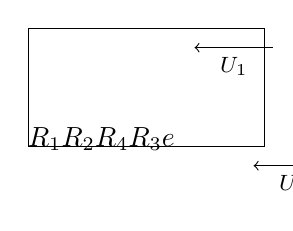
\begin{tikzpicture}[
	scale=1,
	font=\footnotesize,
	]
	\draw (0,0)rectangle(3,1.5);
	\resistanceH{shift={(.75,1.5)}}{$R_1$};
	\resistanceH{shift={(2.25,1.5)}}{$R_2$};
	\resistanceH{shift={(1.5,0)}}{$R_4$};
	\resistanceV{shift={(3,.75)}}{$R_3$};
	\pileL{shift={(0,.5)}}{$e$};
	%tensions
	\draw[shift={(.75,1.5)},<-](-.5,-7pt)--++(1,0)node[midway,below]{$U_1$};
	\draw[->,shorten <=7pt,shorten >=7pt](3,0)--(1.5,1.5)node[midway,left]{$U_2$};
	\draw[shift={(1.5,0)},<-](-.5,-7pt)--++(1,0)node[midway,below]{$U_3$};
\end{tikzpicture}